%%%%%%%%%%%%%%%%%%%%%%%%%%%%%%%%%%%%%%%%%%%%%%%%%%%%%%%%%%%%%%%%%
%  _____       ______   ____									%
% |_   _|     |  ____|/ ____|  Institute of Embedded Systems	%
%   | |  _ __ | |__  | (___    Wireless Group					%
%   | | | '_ \|  __|  \___ \   Zuercher Hochschule Winterthur	%
%  _| |_| | | | |____ ____) |  (University of Applied Sciences)	%
% |_____|_| |_|______|_____/   8401 Winterthur, Switzerland		%
%																%
%%%%%%%%%%%%%%%%%%%%%%%%%%%%%%%%%%%%%%%%%%%%%%%%%%%%%%%%%%%%%%%%%

\chapter{Glitches}\label{chap.glitch}

\section{Definition Glitches}\label{sect.glitch_def}
Im technischem Bereich bedeutet ein Glitch, eine ungewollte, flüchtige Signalspitze, die ein Fehlverhalten im System verursacht (vlg.Cambridge Dictionaire in: \ref{chap.anhang_dictionaire} Definitionen Glitch in english).
Am intuitivsten ist die bildliche Darstellung des Fehlverhaltens (siehe Abbildung \ref{fig.glitch.def}).
\begin{figure}[H]
	\centering
	\includegraphics[width=\textwidth]{images/def_glitch_1.png}
	\caption{Glitch-Signalspitzen}
	\label{fig.glitch.def}
\end{figure}


Das Glitch ist in der digitalen Signalverarbeitung ein bekannter Begriff und wird dort unter anderem leicht sarkastisch beschrieben:\\
Als "Glitch" wird eine ungewollte, flüchtige "Signalspitze" bezeichnet, die Zähler aufwärts zählt, Register löscht oder einen ungewollten Prozess startet." (Fletcher, Digital design, 472).\\

Aus diesem Grund ist es wichtig, diesen Begriff und seine Ursache zu kennen.\\


\section{Ursache für Glitches}\label{sect.glitch_ursache}
Die Urache f\"ur der flüchtigen Spannungsspitzen sind asynchrone Inputs. Alle Prozesse, die nicht getaktet werden (z.B. In- und Output-Logik, direkte Signalzuweisungen) können ungewollte Spannungsspitzen verursachen.In Abbilung \ref{fig.glitch.bild1} verursacht das ungetaktete Eingangssingal Q die Spannungsspitzen, weil das Singal Q zu lange anhält. \\
\begin{figure}[H]
	\centering
	\includegraphics[width=\textwidth]{images/def_glitch_2.png}
	\caption{Ursache f\"ur Glitches}
	\label{fig.glitch.bild1}
\end{figure}



\section{Glitches erzeugen}\label{sect.glitch_detect}
Die erste Aufgabe der Projektarbeit ist, Glitches zu detektieren, um das Phänomen besser verstehen zu können. \\
\subsection{Glitches Aufgrund von Bauteiltoleranzen}\label{sect.glitch_toleranzen}

Der erste Ansatz war, ein Zähler aus 4 Flipflops mit asynchronem Dekoder zu implementieren. Die Erwartung war, dass durch die Bauteiltoleranzen der Flip-Flops die vier Ausgänge an den FlipFlops nicht genau der zu erwartenden nächsten Zahl entspricht, sondern kurzzeitig eine falsche Zahl am Dekoder anliegt.
Dadurch zählt der Dekoder falsch.

\subsubsection{Konzept}
Um die Chance eines falschen Wertes zu erhöhen, werden vier Werte dekodiert: dezimal 3,7,11 und 15. Diese vier Werte folgen in denselben Abständen von 80 ns. Erscheint an den Ausgängen ungewollte eine dieser 4 Zahlen, so werden diese falscherweise dekodiert. Dies falschen Peaks sollten \textit{zwischen} den regelmässigen Abständen auftreten. 
\todo {Totalüberarbeitung  Text Bild: Deodieren 3,7,11,15. Kein RESET.(Blick auf Endlösung)}
\begin{figure}[H]
	\centering
	\includegraphics[width=0.3\textwidth]{images/4_FF.png}
	\caption{RTL Zahler mit asynchronem Dekoder}
	\label{fig.glitch.counter2}
\end{figure}


\subsubsection{Implementation}
\begin{figure}[H]
	\centering
	\includegraphics[width=\textwidth]{images/RTL_counter_2.png}
	\caption{RTL Zahler mit asynchronem Dekoder}
	\label{fig.glitch.counter2}
\end{figure}
\todo {Bild Asynchronem Zähler besser beschreiben}

Um die gewollten Zahlenwerte von den Glitches zu unterschieden, wird das asynchrone Singnal getaktet. Dadurch erscheint der korrekte Zählwert mit einem Takt Verzögerung. Die Periode ist 20 ns (CLK = 50 MHz).\\


\subsubsection{Result}
Der Ansatz, dass die Bauteiltoleranzen der Flip-flops eine Ursache für asynchrone Inputs in den Dekoder sind ist korrekt. Die Umsetzung zeigte sich jedoch als schwierig, da die heutigen Flip-Flops zu schnell sind bzw. ihre Toleranzen zu klein um sichtbar zu werden. \todo {Timeanalyse für FF} Aus diesem Grund entschlüsselte der asynchrone Dekoder trotz kleinen Verzögerungen die Werte stets korrekt.\\


\subsection{Glitches Aufgrund von Pfadverzögerung}\label{sect.glitch_toleranzen}
Der zweite Ansatz ist die gesuchte Bauteilverzögerungen über längere Signalpfade zu simulieren.Der Dekoder des Zählers bleibt asynchron. 

\subsubsection{Konzept}
Dekodiert wird die Zahl 15. Durch intelligentes Routing (FF 1 wird verzögert, FF 2 wird beschleunigt) wird der Zustand der Zahl 11 forcier \todo {Bild FF1 verzögert, FF2 schneller}

\subsubsection{Implementation} 
Cyclone II, Board De2. Quartus 13.0sp.

Die Pfad\textit{verlängerung} wird über das Routing über die GPIO-Pins des Headers 1 gemacht (siehe Abbildung \ref{fig.glitch.routing}. Die obersten vier Doppel-Pins erhalten eine "Brücke", sodass das Signal links ausgegeben und rechts wieder eingespiesen wird.\\
Signal\textit{verkürzung} ist eine direkte Signalzuweisung \todo {korrektes Wort ?(Concourent Assignment)} .\\
\begin{figure}[H]
	\centering
	\includegraphics[width=0.3\textwidth]{images/GPIO_Belegung.png}
	\caption{GPIO Anschlüsse}
	\label{fig.glitch.routing}
\end{figure}

Auf dem KO wird das asynchrone Glitch-Signal und das synchrone Zählersignal neben dem Takt ausgegeben. Weil der Zähler synchronisiert wurde, ist der Wert 1 Periode (= 20 ns) später als der Glitch.\\

\begin{figure}[H]
	\centering
	\includegraphics[width=\textwidth]{images/RTL_glitch_detection_bemalt.png}
	\caption{Zähler mit Signal-Routing über GPIO}
	\label{fig.glitch.routing}
\end{figure}
Im RTL-Diagramm sieht man deutlich den Unterschied zwischen dem asynchronen Zähler, der über das Gate \textit{reset\_{counter}} beim Wert 15 einen Impuls an den Ausgang glitch gibt und dem synchronisierten Zähler \textit{cnt\_{sync}} der dem asynchronen Ausgang nachgeschaltet ist und dieses Signal taktet. Das getaktete Zähl-Signal geht an den Ausgang \textit{count}.

\subsubsection{Result} 
\begin{figure}[H]
	\centering
	\includegraphics[width=0.8\textwidth]{images/Glitch_2_good_kommentar.png}
	\caption{Glitch (gelb), Zähler (grün) und Takt (orange)}
	\label{fig.glitch.result_1}
\end{figure}

Typisch ist, dass der synchrone Zähler eine Signalbreite von genau einer Periode hat, da dieses Signal getaktet ist. Dagegen hat der asynchrone Glitch keine konstante Breite.
\begin{enumerate}
	\item{Bei welchen Zählständen treten Glitches auf?}

	\item{Wie hängen die Zählständen mit dem gewählten Routing zusammen?}

\end{enumerate}
	
